% Created 2024-08-06 Tue 15:13
% Intended LaTeX compiler: pdflatex
\documentclass[presentation]{beamer}
\usepackage[utf8]{inputenc}
\usepackage[T1]{fontenc}
\usepackage{graphicx}
\usepackage{longtable}
\usepackage{wrapfig}
\usepackage{rotating}
\usepackage[normalem]{ulem}
\usepackage{amsmath}
\usepackage{amssymb}
\usepackage{capt-of}
\usepackage{hyperref}
\usetheme{Darmstadt}
\author{Louis}
\date{\today}
\title{}
\hypersetup{
 pdfauthor={Louis},
 pdftitle={},
 pdfkeywords={},
 pdfsubject={},
 pdfcreator={Emacs 29.3 (Org mode 9.6.15)}, 
 pdflang={English}}
\begin{document}

\begin{frame}{Outline}
\tableofcontents
\end{frame}

\section{Reviewed survey papers}
  \subsection{Nauta et al. 2023}
  \subsection{Mohensi et al. 2021}
  \subsection{Das \& Rad 2020}
  \subsection{Schwalbe \& Finzel 2023}
\section{Paper collection}
  \subsection{Broad search with database}
  \subsection{Iterative search}
\section{Methodology}
  \subsection{Paper categorization}
  \subsection{What to evaluate?}
\section{Organization}
  \subsection{Create own knowledge database (from dblp)}
  \subsection{Workflow}

\begin{frame}[label={sec:org030fe25}]{Nauta et al. 2023}
\begin{block}{Paper Selection}
\begin{itemize}
\item Literature from 2014-2020
\item 12 conferences
\item Query: explain*|explanat*|interpret*
\item Search on 04.05.2021: 606 Results
\item Without workshop papers and tutorials: 494
\item After inclusion criterion 361:
\end{itemize}
\begin{quote}
Original work introducing, applying, and/or evaluating one or more methods for explaining a machine
learning model.
\end{quote}
\begin{itemize}
\item only papers that introduce a new xai technique: 312
\begin{itemize}
\item the reduced 49 papers were still concidered for evaluation metrics
\end{itemize}
\end{itemize}
\end{block}
\end{frame}
\begin{frame}
\begin{block}{Categorization of the papers}
There were 6 dimensions for paper categorization:
\begin{itemize}
\item Type of data (time series, graph, image\ldots{})
\item Type of predictive model (NN, SVM, Tree Ensemble\ldots{})
\item Type of method used for to explain (built-in, post-hoc\ldots{})
\item Type of explanation (Heatmap, Feature Plot\ldots{})
\item Type of problem (Model explanation, outcome explanation\ldots{})
\item Type of task (classification, regression\ldots{})
\end{itemize}
\end{block}
\end{frame}
\begin{frame}
\begin{block}{XAI Explanation Quality Properties}
The authors defined 12 quality properties to be examined:
\begin{itemize}
\item Correcteness
\item Completeness
\item Consistency
\item Continuity
\item Contrastivity
\item Covariate complexity
\item Compacteness
\item Composition
\item Confidence
\item Context
\item Coherence
\item Controllability
\end{itemize}
\end{block}
\end{frame}
\begin{frame}
\begin{block}{General}
\begin{itemize}
\item Extensive approach focusing on finding trends and maybe blindspots in research
\item Due to the high volume, statistic evaluation is possible
\item Points to automated, quantitative evaluation methods (could be interesting for us -> TimeXAI)
\item Maybe cherry-pick from their quality properties?
\end{itemize}
\end{block}
\end{frame}

\begin{frame}[label={sec:org1393c3e}]{Mohseni et al 2021}
\begin{block}{Paper Selection}
\begin{itemize}
\item choose from multiple disciplines: ML, HCI, Visualization, Psychology
\item iterative approach chosing 40 papers as a start and then doing upwards/downwards literature research with some refinement, resulting in 226 papers
\item keywords: interpretability, explainability, intelligibility, transparency, algorithmic decision-making, fairness, trust, mental model, and debugging in machine learning and intelligent systems
\end{itemize}
\end{block}
\end{frame}
\begin{frame}
\begin{block}{Summary}
\begin{itemize}
\item derived a general framework from a more "distanced" view for a whole design process of an XAI system used by novices and experts alike
\item split design goals between novice users, data experts and AI experts
\item Introduce 5 evaluation measures for XAI systems
\item In general more HCI view
\end{itemize}
\end{block}
\end{frame}
\begin{frame}
\begin{block}{General}
\begin{itemize}
\item HCI view might be interesting for TimeXAI, do we want to incorporate this?
\item iterative approach maybe interesting for us?
\item cherry-pick goals and evaluation measures?
\end{itemize}
\end{block}
\end{frame}

\begin{frame}[label={sec:org8fdd490}]{Das \& Rad 2020}
\begin{block}{Paper selection:}
\begin{itemize}
\item focuses on milestone papers from the last 15 years
\item good overview over most interesting papers
\end{itemize}
\end{block}
\begin{block}{Main categorization:}
\begin{itemize}
\item Scope: Local/global explanations
\item Methodology: Perturbation/Backpropagation
\item Usage: Model-intrinsic/post-hoc
\end{itemize}
\end{block}
\end{frame}
% \begin{frame}
% \begin{block}{Definitions:}
% \begin{itemize}
% \item Interpretability
% \item Interpretation
% \item Explanation
% \item white-box
% \item black-box
% \item transparent
% \item Trustability
% \item Bias
% \item Fairness
% \end{itemize}
% \end{block}
% \end{frame}
\begin{frame}
\begin{block}{Summary:}
\begin{itemize}
\item compares XAI methods directly based on methodology
\item most research focuses on model-agnostic post-hoc explainability due to easy integration and wide reach
\end{itemize}
\end{block}
\end{frame}

\begin{frame}[label={sec:org7e81ca3}]{Schwalbe \& Finzel 2023}
\begin{itemize}
\item Reviewed 50 surveys on XAI in meta survey
\item there is no definite taxonomy for XAI
\item they tried to introduce one (pretty recent 01/2023), maybe we can adapt to this?
\end{itemize}
\end{frame}

\begin{frame}[label={sec:orgedcff66}]{Paper collection:}
\begin{block}{Large scale approach with database}
\begin{table}
\centering
\begin{tabular}{p{0.4\linewidth} | p{0.4\linewidth}}
 Pros & Cons  \\\hline
 * captures most papers and will result in an extensive amount of data & * filtering and reading will be a lot of work \\
 * if done with a database approach might be a start for a knowledge database for the future & * worst case: many papers are not insignificant (=can't be discarded) but also not helpful \\
 * enables statistic analysis &  \\
 * best chances to get impulses for TimeXAI & 
\end{tabular}
\end{table}
\end{block}

\begin{block}{Iterative approach}
+ hopefully less "bad" papers to read and include\\
+ easier to focus on specific area in current research (e.g. time series)\\
- where to start? Finding a start will take time (maybe look at Das \& Rad 2020)\\
- higher chance to miss important/interesting papers\\
\end{block}
\end{frame}

% \begin{frame}[label={sec:orgd64282c}]{Methodology:}
% \begin{itemize}
% \item We limit data to time series
% \item Do we need other limitations?
% \end{itemize}
% \begin{block}{Paper categorization:}
% \begin{itemize}
% \item More specific categorization e.g. Nauta et. al.
% \end{itemize}
% \begin{figure}[htbp]
% \centering
% 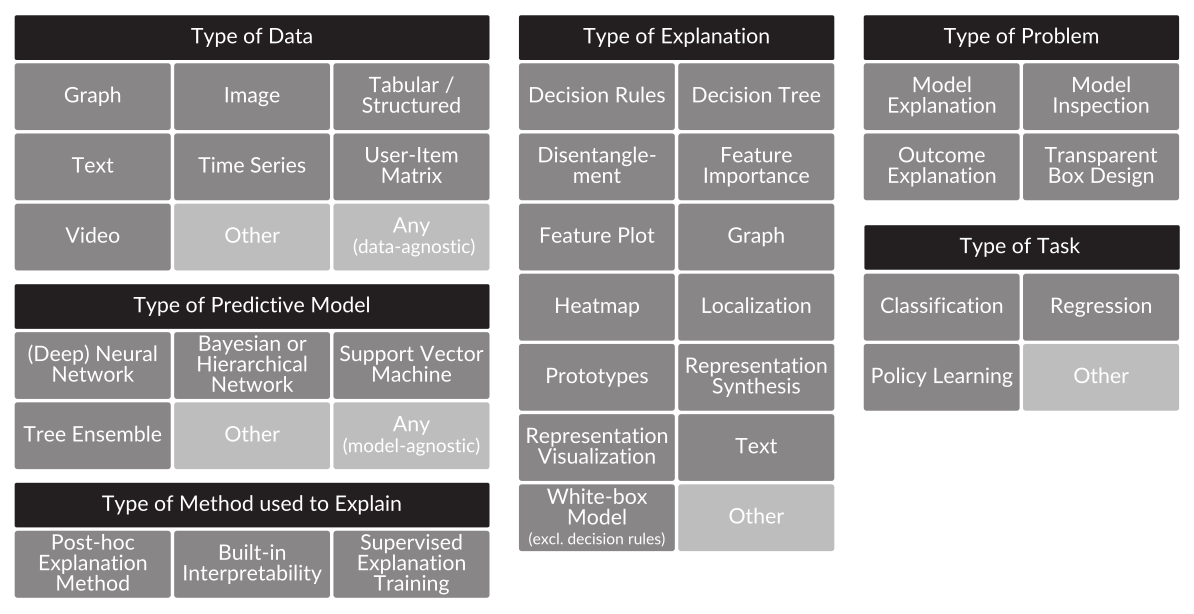
\includegraphics[width=.9\linewidth]{./NautaCategorization.png}
% \caption{\label{fig:org2ab648d}Categorization by Nauta et. al.}
% \end{figure}
% \begin{itemize}
% \item More general categorization e.g. Das \& Rad
% \end{itemize}
% \begin{figure}[htbp]
% \centering
% 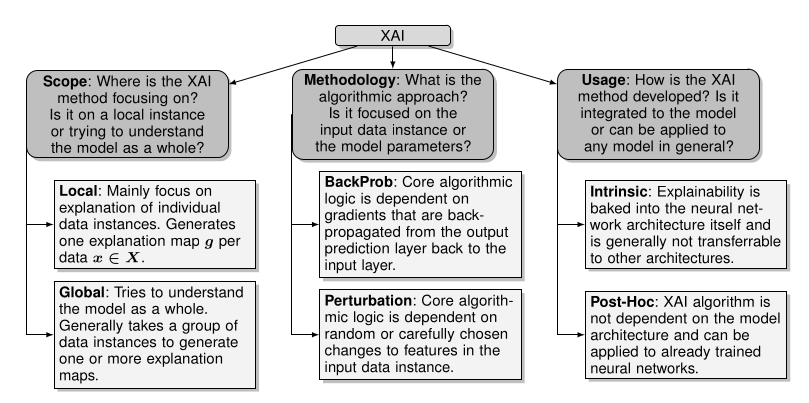
\includegraphics[width=.9\linewidth]{./DasRadCategorization.png}
% \caption{\label{fig:org646751b}Categorization Das \& Rad}
% \end{figure}
% \end{block}

% \begin{block}{What to evaluate?}
% \begin{itemize}
% \item currently many surveys seem to struggle with taxonomy e.g. what is a "good" explanation and try to define qualaties for what is considered good
% \item Stems more from HCI perspective, do we focus on it and how extended?
% \item A (good?) overview is extracted by Schwalbe \& Finzel
% \end{itemize}

% \begin{figure}[htbp]
% \centering
% 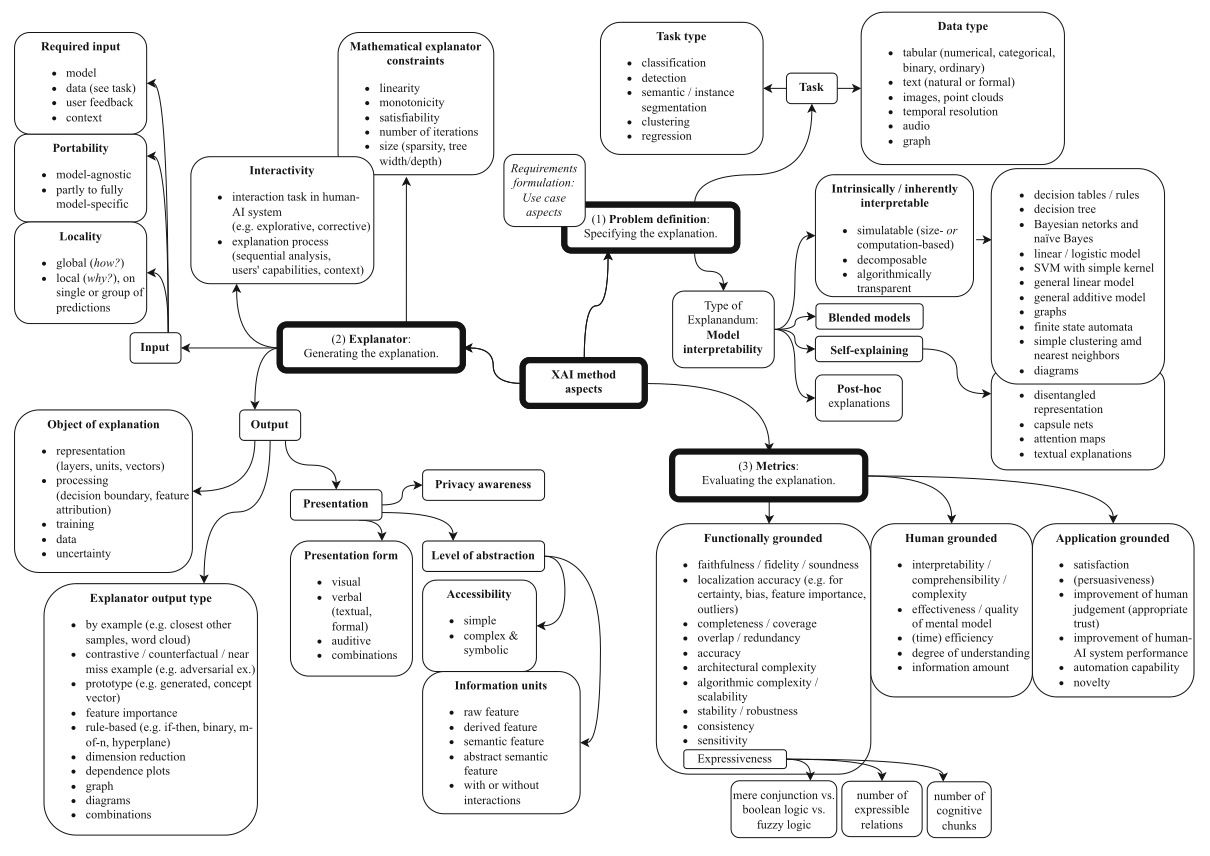
\includegraphics[width=.9\linewidth]{./SchwalbeFinzelTaxonomy.png}
% \caption{\label{fig:orgfc3dda4}Taxonomy by Schwalbe and Finzel}
% \end{figure}
% \end{block}
% \end{frame}
\end{document}
